\setstretch{1.6}
\sectiontitle{6}{Software Refactoring}
\lhead{Software Refactoring} % section header
As mentioned introduction wise, this thesis builds upon the work and code developed for a previous iteration of the system. However, the control code, implemented in C++ using Qt, lacked the structure and readability to allow for the expansions necessary for this thesis. There was clear room for improvement especially when it came to modularization, exemplified by the MainWindow class that managed several distinct functionalities and over 80 different member variables. Therefore, before continuing on with the project a full refactoring of the code was necessary. The objective was to save time in the long run by creating modular, robust, readable code that could easily be further built upon and used in future projects.

\lhead{Software Refactoring - Theory} % section header
\subsection{Theory}
\subsubsection{Software architecture for real-time systems}
Real-time systems require software that is predictable and responsive, even under strict timing constraints. This places additional demands on the software design, especially since codebases for such system may grow rapidly when there is necessity for GUI handling, hardware commands, control calculations and communication protocols. According to McConnel \cite{steve_mcconnell_code_nodate}, high-quality architecture in such systems should emphasize simplicity, clarity, and robustness to change. 
\newline \newline
A well-structured architecture improves maintainability and extensibility by making the system easier to understand and reason about. In real-time contexts, this often translates into an architecture that minimizes dependencies betwen components and provides clear seperation between hardware interaction, control logic, and application-level coordination \cite{tanenbaum_distributed_2007}.

\subsubsection{Modular design principles}
Modularity is one of the most important design principles when managing software complexity. Modular systems break down functionality into discrete units that encapsulate behavior and expose minimal interfaces \cite{steve_mcconnell_code_nodate}. This separation reduces the mental burden on developers and allows individual parts of the system to be developed, tested, and modified independently—greatly improving maintainability and scalability.
\newline \newline
Effective modularity hinges on two key design goals: low coupling and high cohesion. Low coupling refers to moules having minimal dependencies on each other, and high cohesion means that all parts fo a module contribute to a single, clear purpose \cite{steve_mcconnell_code_nodate}. These ideas build on the concept of "information hiding" \cite{parnas_criteria_1972} where internal implementation details are kept private, preventing unintended interactions across modules.

\subsubsection{Threading and concurrency}
Concurrency is often necessary in real-time systems to meet iming constraints and maintain responsiveness. Use of threads allows the system to perform multiple tasks concurrently, such as sensor data acquisition, visualization, control loop comuptation and user interaction, without blocking the main execution path.
\newline \newline
However, introducing concurrency also introduces complexity. Issues such as race conditions, deadlocks and nondeterministic behavior must be managed. McConnell \cite{mcconnell_code_2004} warns that improperly designed concurrency can reduce the reliability of software rather than improve performance. Therefore, concurrent systems should be built using clear a clear design, thead-safe communication mechanisms and minimal shared states \cite{noauthor_software_nodate}.

\subsubsection{Event-driven communication in Qt}
A common and reliable pattern for concurrent real-time systems is event-driven communication between threads. In this model, components communicate through asynchronous messages rather than direct calls or shared varieables. In Qt this is implemented via the signal-slot mechanism. Signals are emitted when events occur, and slots (connected handler functions) respond to those events. Qt ensures that the communication is thread safe by searializing signal delivery using the vent loop of the receiving thread, meaning that it will execute in the context of the receiving threads event loop. 

\lhead{Software Refactoring - Methods} % section header
\subsection{Methods}
\subsubsection{Analysis of the original code base}
The refactoring process began with a thorough analysis of the existing codebase. The existing methods and classes were documented and their interactions were visualized in figure such as \ref{fig:oldarchitecture}.
\begin{figure} [H]
    \centering
    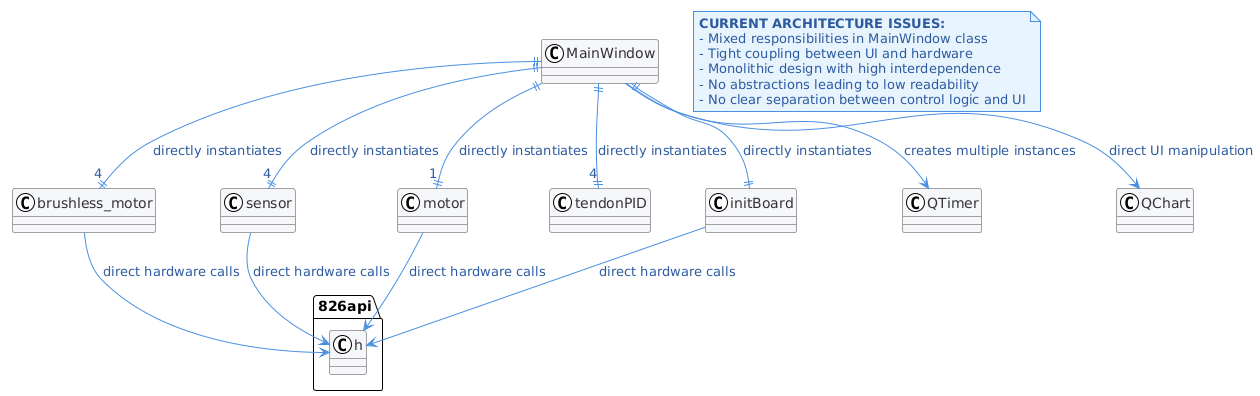
\includegraphics[width=1.1\linewidth]{images/Software documentation/old code/architecture2.png}
    \caption{Original architecture, prior to refactoring}
    \label{fig:oldarchitecture}
\end{figure}
 \begin{wrapfigure}{r}{0.45\textwidth}
    \centering
    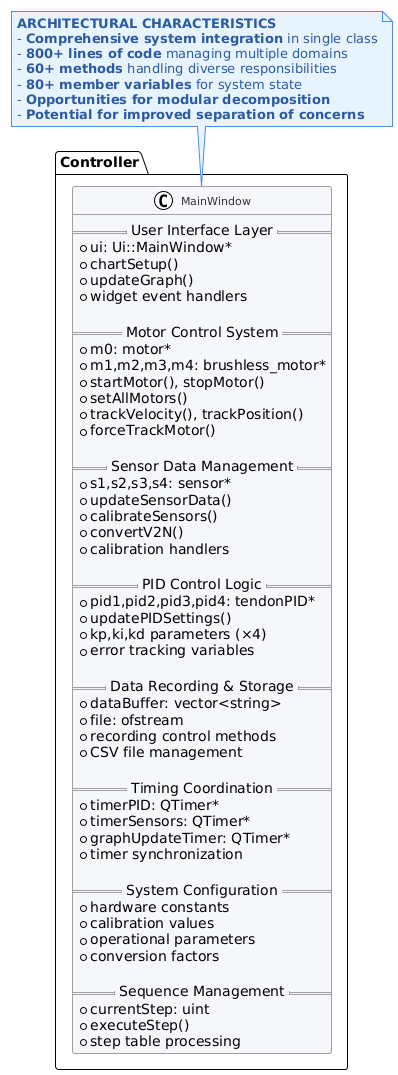
\includegraphics[width=\linewidth]{images/Software documentation/old code/mainwindow2.png}
    \caption{\texttt{MainWindow} implementation, prior to refactoring}
    \label{fig:oldmainwindow}
\end{wrapfigure}This step provided an overview of the software architecture and highlighted areas where the structure violated modular design principles, such as excessive coupling and low cohesion. 

An analysis of the original codebase revealed that the main issue was the low cohesion and large amount of responsibilities and data managed by the \texttt{MainWindow} class, as is exemplified in figure \ref{fig:oldmainwindow}. It also showed that even though the original architecture seen in \ref{fig:oldarchitecture} looks seemingly modularized into relevant modules such as \texttt{motor} and \texttt{tendonPID}, those classes did not in reality have ownership of the appropriate methods or data. The elements that should have been implemented in those classes largely remained in the \texttt{MainWindow} class. This resulted in high interdependence, with little abstraction and low readability of the code.

\subsubsection{Restructuring Methodology}
Based on the architectural guidelines described in the theory section, a revised design was developed. The design emphasizes smaller highly cohesive classes and separation of concerns by defining minimal, well-documented interfaces between modules and isolating hardware-dependent functionality, for different types of application level logic. The existing code was refactored to fit into this structure and unnecessary functionality was removed. Existing errors in the code were also remedied. Thereafter new code was written into the the modules in order to expand the functionality of the system.

\lhead{Software Refactoring - Results} % section header
\subsection{Results}

\subsubsection{Modularization}
The code was restructured into well defined classes, each responsible for a specific task. These classes were further grouped into folders, these folders are very briefly described in the table below. However a description however of all the classes can be found in the appendix. 

\begin{table}[htbp]
\centering
\caption{High Level Descriptions of Software Folder Organization}
\begin{tabular}{p{0.3\textwidth}p{0.65\textwidth}}
\toprule
\textbf{Module} & \textbf{Description} \\
\midrule
Root Directory & Main application framework includes \texttt{MainWindow}, \texttt{Logger}, \texttt{sensor}, and classes responsible for running specific sequences such as \texttt{Tester} and \texttt{AirCalibrator}. \\
\addlinespace
Motor Control & Hardware control modules for linear stage positioning and brushless motor actuation with motion estimation. \\
\addlinespace
Tendon PID Control & Closed-loop tension control system managing individual tendon forces through coordinated PID controllers. \\
\addlinespace
Vision System & Communication interface with Python-based vision system for real-time tip tracking and recording control via ZeroMQ messaging. \\
\addlinespace
Path Following & Trajectory planning and guidance algorithms including line-of-sight navigation, feedback control, and curvature-to-tension mapping. \\
\bottomrule
\end{tabular}
\end{table}

\subsubsection{Architecture}
A visualization of the resulting architecture after refactoring can be seen in figure \ref{fig:architecture}. As shown, the system in now organized into modular, loosely coupled components with clear responsibilities. The architecture is also layered, with lower-level modules (such as hardware control and above that tendonpids) forming the foundation for higher-level logic (such as path following).

\begin{figure} [H]
	\centering
	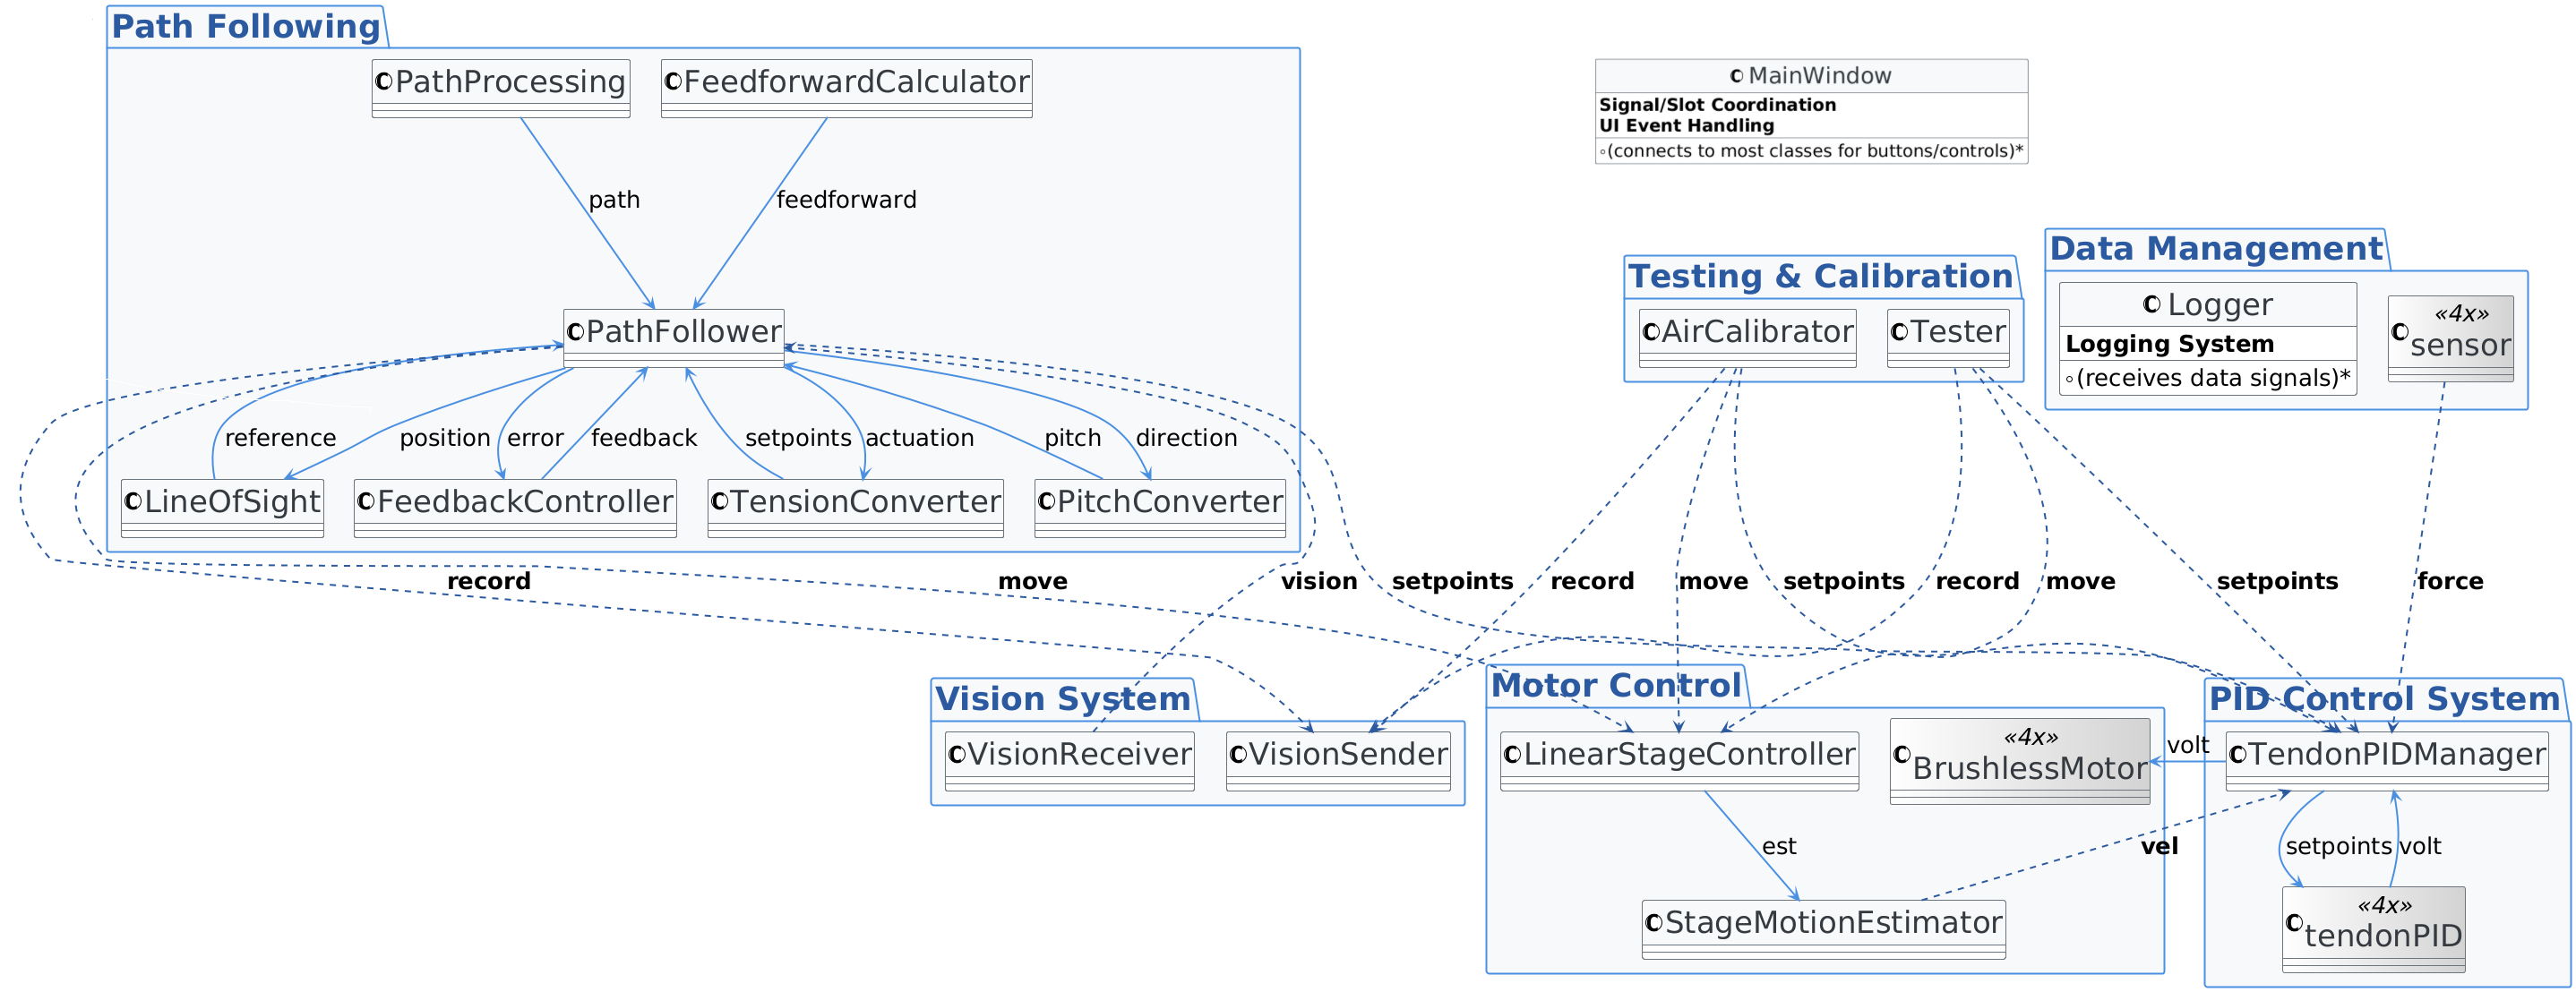
\includegraphics[width=1.1\linewidth]{images/Software documentation/architecture3.png}
	\caption{Final control code base architecture after refactoring}
	\label{fig:architecture}
\end{figure}




\subsubsection{Threading}
The entire system follows and event-driven architecture using Qt's signal-slot mechanisms wherever possible. This reduces the need for extensive multithreading as modules do not block threads for long periods. Instead most classes react to signals or timers. Some components, such as sensor data acquisition and closed-loop tension control, operate on fixed update intervals using timers. Others, like the path-following controller are triggered by receiving a new vision measurement.
\begin{figure} [h]
    \centering
    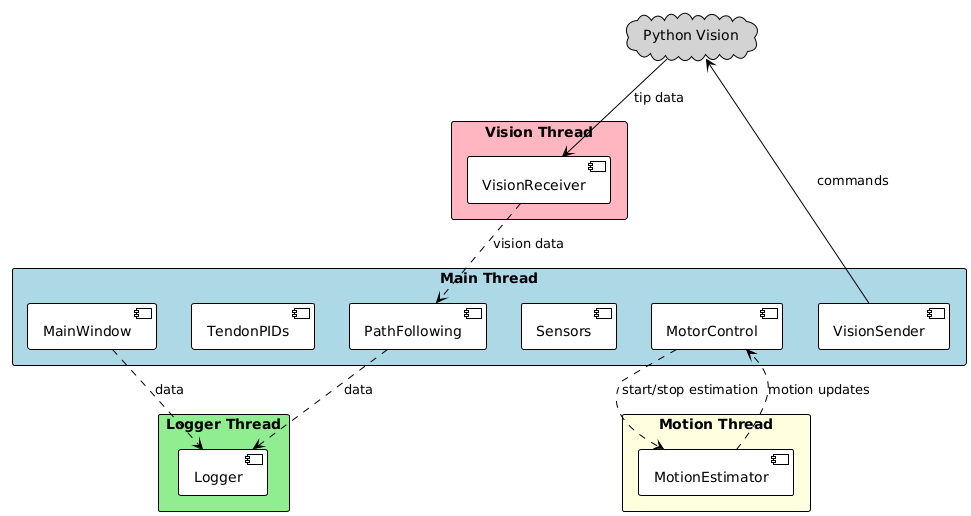
\includegraphics[width=0.95\linewidth]{images/Software documentation/threads.png}
    \caption{Visualization of communicaion between the 4 threads of the control system}
    \label{fig:threads}
\end{figure}
To support real-time performance and responsiveness, multithreading was introduced where strictly necessary. Only components that demonstrated clear performance bottlenecks or responsiveness issues were moved to separate threads. The components run in dedicated threads outside of the main thread are described in the following table. Addittionally a simple figure visualizing of the threads and the signals sent between them can be seen in figure \ref{fig:threads}

\begin{table}[htbp]
\centering
\caption{Threading Architecture Description}
\begin{tabular}{p{0.3\textwidth}p{0.65\textwidth}}
\toprule
\textbf{Thread} & \textbf{Description} \\
\midrule
Logging Thread & Records sensor and control data without blocking the main loop. \\
\addlinespace
Motion Estimation Thread & Continuously estimates stage speed at a high frequency while the linear stage is running for use in feedforward for the closed loop tension control. \\
\addlinespace
Vision Receiver Thread & Continuously listens for incoming vision data and receives and parses it. \\
\bottomrule
\end{tabular}
\end{table}

\subsubsection{Graphical-User-Interface}








\subsection{Discussion}


By combining lightweight threads for parallel execution with queued, thread-safe communication via Qt signals/slots, real-time systems can achieve both responsiveness and reliability without falling prey to classic concurrency pitfalls.

Only components that demonstrated clear performance bottlenecks or responsiveness issues were moved to separate threads. This approach minimizes complexity while still meeting the system’s real-time requirements. Communication between modules is kept minimal and modular, consistent with the design principles of low coupling, high cohesion, and information hiding discussed in the theory section.

The result is a system that is easier to maintain, extend, and test, with clear module boundaries and a simplified control flow.

By relying on Qt’s signal-slot mechanism, the system maintains responsive behavior while keeping communication between modules clean, thread-safe, and loosely coupled.

This approach allows the system to meet its real-time requirements while maintaining simplicity and modularity in both structure and execution flow.


The architectural refactoring successfully addressed the limitations of the original monolithic codebase, resulting in significant improvements in software quality and system performance.
The modularization effort created a well-structured codebase with clear separation of concerns. Each module now has a single, well-defined responsibility, making the code significantly more maintainable and extensible. The logical folder organization provides intuitive navigation and reduces code coupling while increasing cohesion.
The event-driven architecture using Qt's signal-slot mechanism eliminated blocking operations in the main thread, resulting in a responsive user interface. The selective use of multithreading for performance-critical components ensured real-time requirements were met without unnecessary complexity. The main control loop now maintains consistent timing with sensor data acquisition, motion estimation, and vision processing running independently.
The dedicated threading architecture enables each subsystem to operate at its optimal frequency. The motion estimation thread achieves high-frequency updates for accurate feedforward control, while the vision receiver thread ensures continuous data flow. The logging thread prevents data recording from impacting control loop timing, maintaining system determinism.
The modular design facilitates easy integration of new components through standardized interfaces. This allows component replacement or enhancement without affecting other system parts. The separation of concerns improved system stability by isolating component failures and preventing cascading effects. These architectural improvements provided a solid foundation for implementing advanced control algorithms while maintaining code clarity and development efficiency.

Each module exposes a minimal interface, making it easier to test, maintain, and reuse individual parts of the system.



